\documentclass[12pt,letterpaper,twocolumn,openany,nodeprecatedcode,bg=none]{dndbook}
\usepackage[english]{babel}
\usepackage[utf8]{inputenc}
\usepackage{longtable,booktabs,array}
\usepackage{calc}
\usepackage{etoolbox}
\usepackage{caption}
\AtBeginEnvironment{longtable}{\small}

% Fix for Pandoc 3.1.7+ image handling
\providecommand{\pandocbounded}[1]{#1}

% Pandoc's compact list helper
\providecommand{\tightlist}{%
  \setlength{\itemsep}{0pt}\setlength{\parskip}{0pt}}

% Remove "Figure N:" prefix from captions
\captionsetup{labelformat=empty}

% Remove section numbering
\setcounter{secnumdepth}{0}

\begin{document}

\title{Ranger}
\author{Class Handbook}
\date{}
\maketitle

\onecolumn

\emph{Your trusty class handbook for the Old Scrolls roleplaying game.}

\clearpage

\begin{figure}
\centering
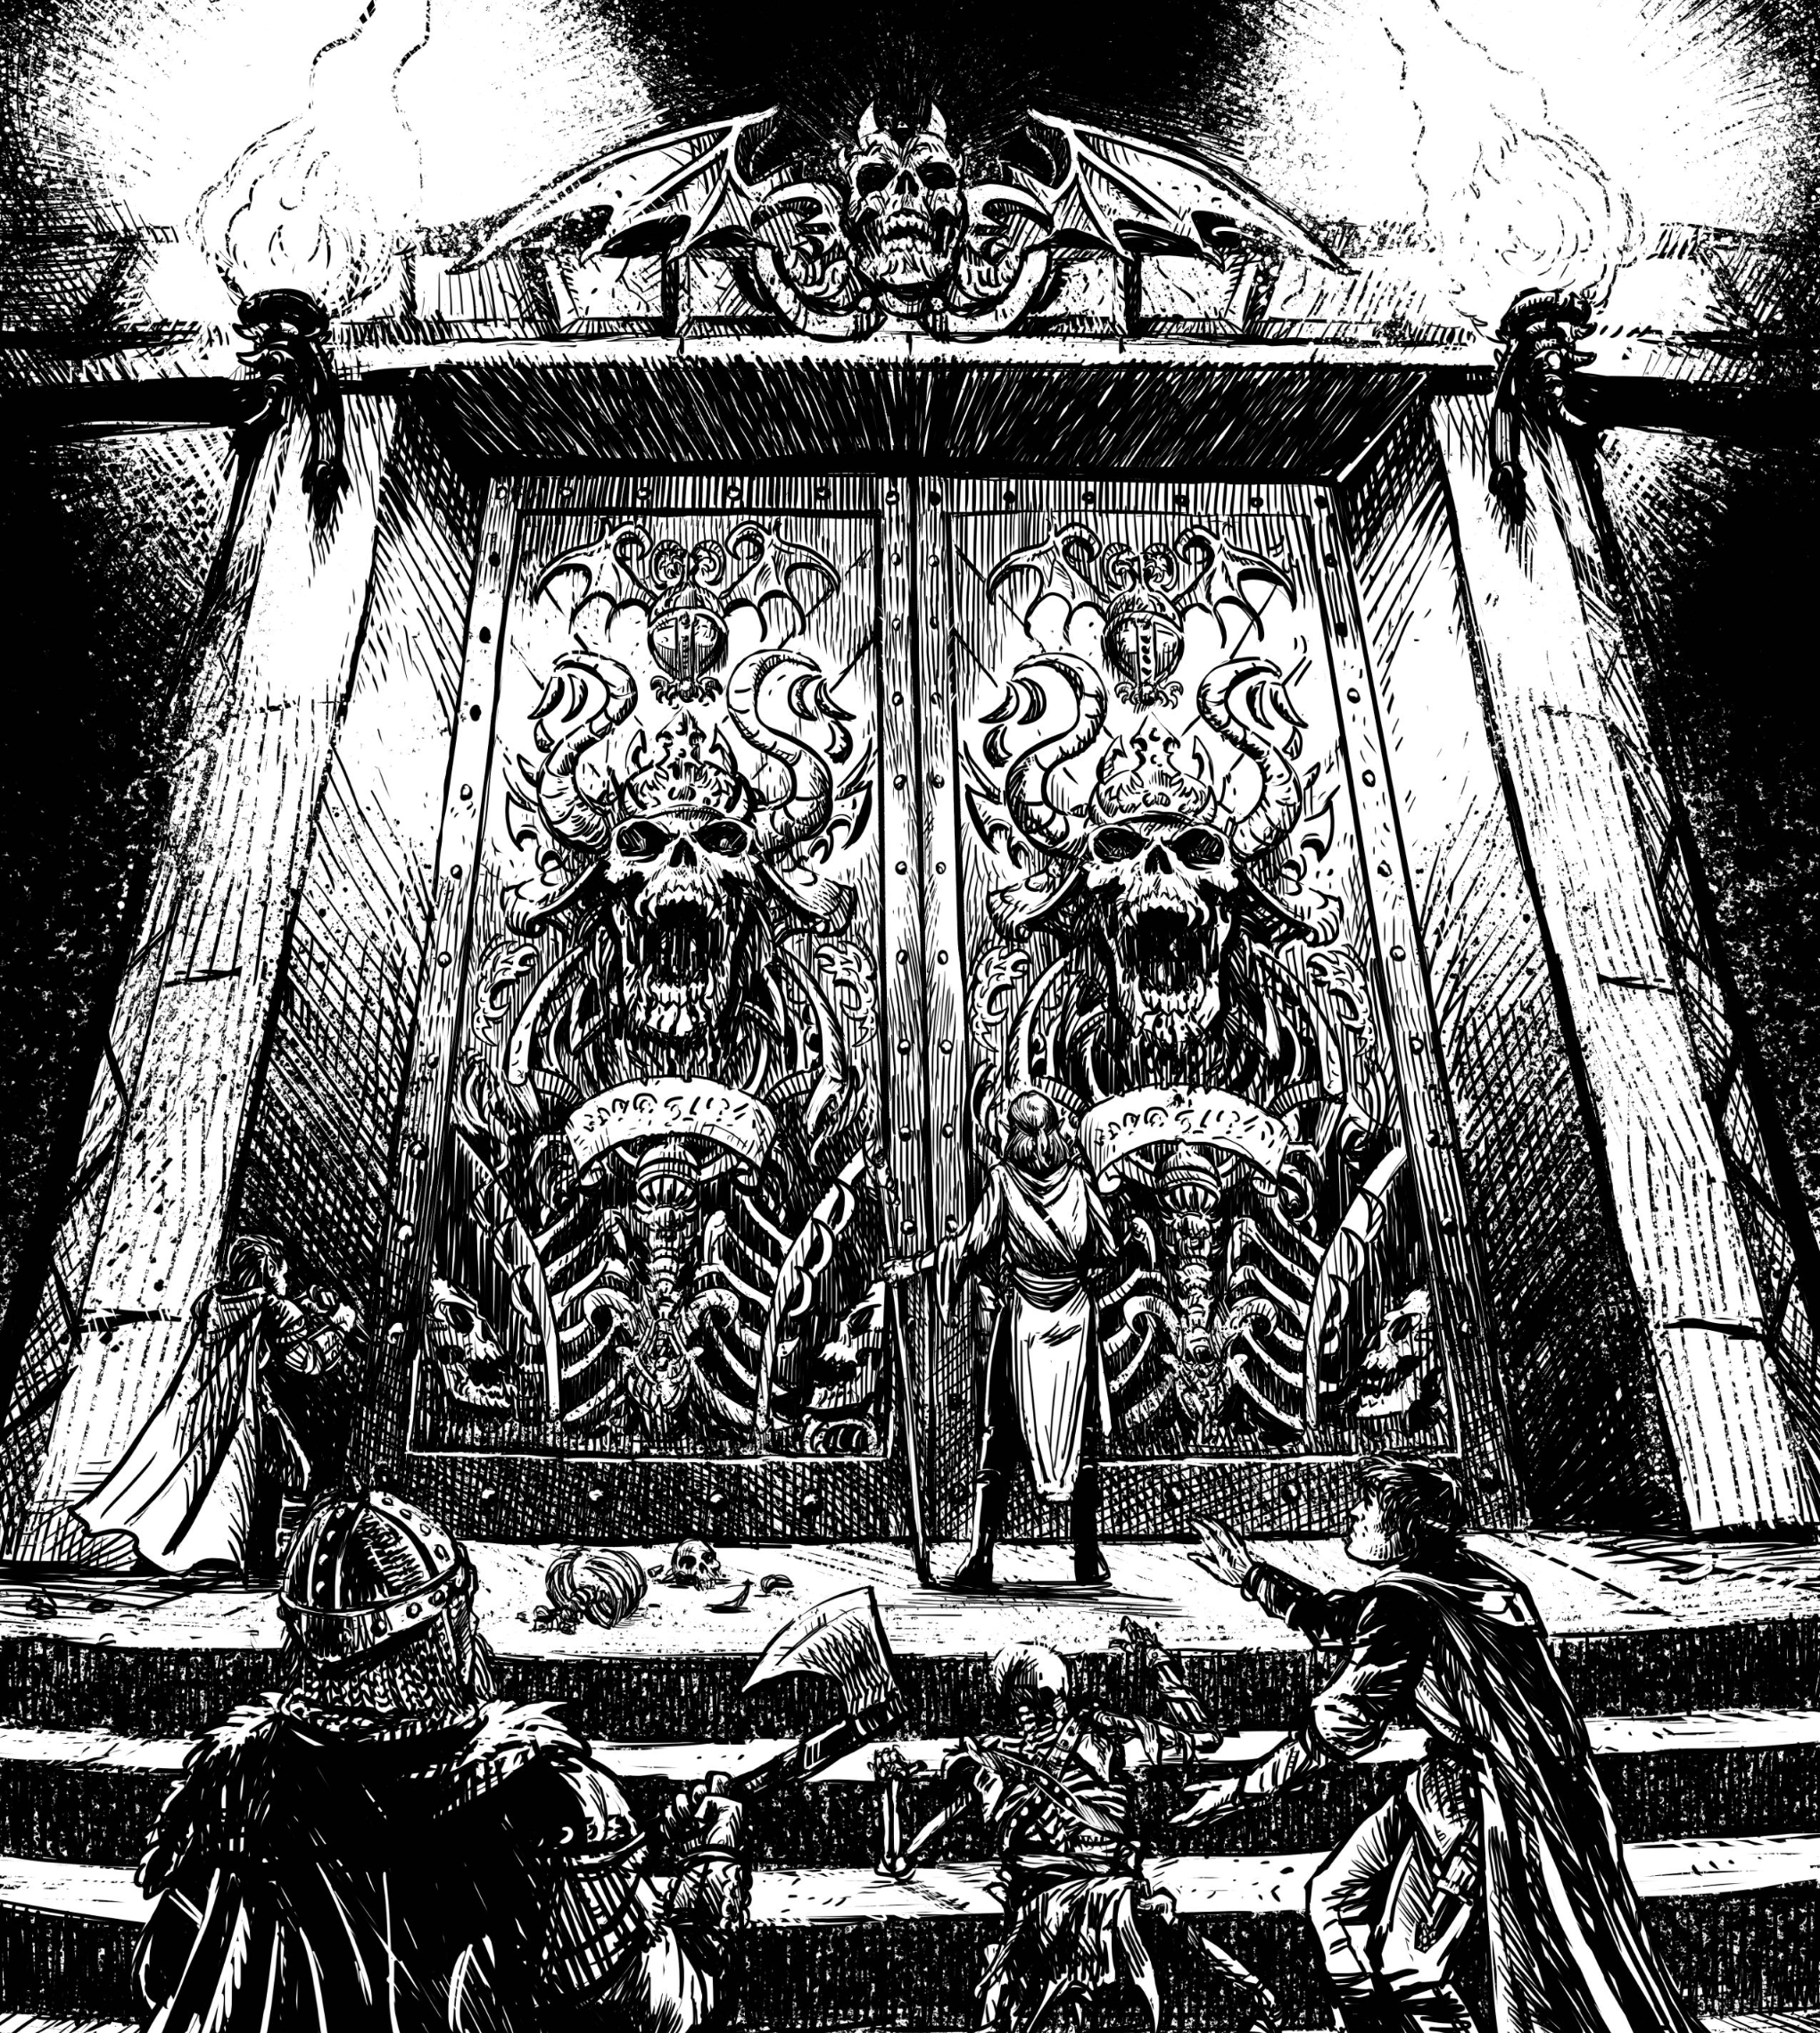
\includegraphics[width=1\linewidth,height=\textheight,keepaspectratio]{dungeonDoor.png}
\caption{\emph{A ranger leads their allies into the unknown}}
\end{figure}

\clearpage

\section{Ranger}\label{ranger}

The ranger is a natural leader, someone who is at home in the wilds and
attuned with nature. They have learned how to form strong bonds with the
beasts of the wilds, and know how to help their allies in times of need.

\subsection{Core Ranger Traits}\label{core-ranger-traits}

\begin{longtable}[]{@{}
  >{\raggedright\arraybackslash}p{(\linewidth - 2\tabcolsep) * \real{0.2542}}
  >{\raggedright\arraybackslash}p{(\linewidth - 2\tabcolsep) * \real{0.7458}}@{}}
\toprule\noalign{}
\begin{minipage}[b]{\linewidth}\raggedright
\textbf{Primary Ability}
\end{minipage} & \begin{minipage}[b]{\linewidth}\raggedright
Dexterity
\end{minipage} \\
\midrule\noalign{}
\endhead
\bottomrule\noalign{}
\endlastfoot
\textbf{Hit Points} & 12 at 1st level, 8 per level gained after 1st \\
\textbf{Saving Throw Proficiencies} & Strength, Dexterity \\
\textbf{Skill Proficiencies} & Choose any 4 skills. If you choose a
skill you already have, you gain expertise with it. \\
\textbf{Weapon Proficiencies} & Choose 3: Blade, Blunt, Bow, Mechanical,
Polearm, and Shield \\
\textbf{Starting Equipment} & Padded Jacket, Longbow, Sabre, Small
Shield, Self-made Map \\
\end{longtable}

\subsection{Ranger Features Table}\label{ranger-features-table}

\begin{longtable}[]{@{}lll@{}}
\toprule\noalign{}
Level & Proficiency & Class Features \\
\midrule\noalign{}
\endhead
\bottomrule\noalign{}
\endlastfoot
1 & +2 & Animal Companion, Wildcraft \\
2 & +2 & Bounding Movement, Ranger's Guidance \\
3 & +2 & Explorer's Talent, Guardian of Nature (d6) \\
4 & +2 & Ability Score Improvement, Wildcraft \\
5 & +3 & Extra Attack, Guardian of Nature (d8) \\
6 & +3 & Ability Score Improvement, Wildcraft \\
7 & +3 & Companion Talent \\
8 & +3 & Ability Score Improvement, Wildcraft \\
9 & +4 & Guardian of Nature (d10) \\
10 & +4 & Boundless Steps \\
\end{longtable}

\twocolumn

\subsection{Ranger Features}\label{ranger-features}

As a ranger, you gain the following class features when you reach the
specified levels. These features are listed on the Ranger Features
table.

\subsection{Level 1: Animal Companion}\label{level-1-animal-companion}

You gain the services of an animal companion, a beast with a mystic
connection to you. You and the beast have an intuitive connection. If
you can see or hear each other, you use body language and subtle sounds
to communicate as if you shared a language.

The selection of animal companions is provided at the end of the class
description. The companion's stats are based on your level.

If your companion dies, you must spend a week wandering the wilds alone
to track down and befriend a new companion.

Your companion is effectively a second character you control. It has
free will but has chosen to ally with you, but you as a player decide
its actions, attitudes, and beliefs. It rolls initiative, takes turns,
and otherwise acts independently.

\subsection{Level 1: Wildcraft}\label{level-1-wildcraft}

Your expertise in woodcraft and exploration allows you to hone your
skills in combat and as a leader. You gain two wildcraft feats of your
choice. When you gain a level, you can swap any wildcraft feat you chose
for another.

\subsection{Level 2: Bounding Movement}\label{level-2-bounding-movement}

You are agile on your feet and difficult to corner. On your turn, you
can move two times.

\subsection{Level 2: Ranger's Guidance}\label{level-2-rangers-guidance}

When you make a check, you can provide guidance to your allies. Until
your next turn, friendly creatures within 30 feet of you can use your
result in place of rolling that same check.

\subsection{Level 3: Explorer's Talent}\label{level-3-explorers-talent}

You are adept at crafting campsites and finding the perfect place to
rest. You can find safe havens in standard wilderness where you can gain
the benefits of extended downtime.

\subsection{Level 3: Guardian of
Nature}\label{level-3-guardian-of-nature}

You gain a guardian die, a d6 you can use in the following ways once per
turn:

\begin{itemize}
\tightlist
\item
  You can roll one die and add it to a damage roll made by you or your
  animal companion. The die's damage type is one of the roll's types of
  your choice.
\item
  You can roll one die and add it to a test you or a creature within 30
  feet of you makes. You choose to add this die after you learn the
  test's result, potentially turning failure into a success.
\end{itemize}

Once you use your guardian die, you can't use it again until your next
turn. Your guardian die becomes a d8 at level 5 and a d10 at level 9.

\subsection{Level 4: Ability Score
Improvement}\label{level-4-ability-score-improvement}

You gain a +1 bonus to two abilities of your choice.

\subsection{Level 4: Wildcraft}\label{level-4-wildcraft}

You gain a wildcraft feat of your choice. When you gain a level, you can
swap any wildcraft feat you chose for another.

\subsection{Level 5: Extra Attack}\label{level-5-extra-attack}

You can attack twice instead of once whenever you take the attack action
on your turn.

\subsection{Level 6: Ability Score
Improvement}\label{level-6-ability-score-improvement}

You gain a +1 bonus to two abilities of your choice.

\subsection{Level 6: Wildcraft}\label{level-6-wildcraft}

You gain a wildcraft feat of your choice. When you gain a level, you can
swap any wildcraft feat you chose for another.

\subsection{Level 7: Companion Talent}\label{level-7-companion-talent}

Your companion gains one of the following benefits. If you gain a new
companion, you can pick a new benefit for it to replace the one you
chose for your former companion.

\begin{itemize}
\tightlist
\item
  \textbf{Iron Hide.} Your companion gains +2 AC.
\item
  \textbf{Skilled.} Pick a skill. Your companion doubles its test bonus
  when making checks that use that skill.
\item
  \textbf{Toughness.} While your companion is at half hit points or
  less, it regains hit points equal to half your level at the end of its
  turn.
\item
  \textbf{Vicious.} Your companion gains a bonus to damage rolls equal
  to half your level.
\end{itemize}

\subsection{Level 8: Ability Score
Improvement}\label{level-8-ability-score-improvement}

You gain a +1 bonus to two abilities of your choice.

\subsection{Level 8: Wildcraft}\label{level-8-wildcraft}

You gain a wildcraft feat of your choice. When you gain a level, you can
swap any wildcraft feat you chose for another.

\subsection{Level 10: Boundless Steps}\label{level-10-boundless-steps}

You now can move three times on your turn.

\onecolumn

\section{Animal Companions}\label{animal-companions}

There are three basic companions you can choose from. Animal companions
are size Medium beasts unless otherwise noted. Their level equals yours
and they share your alignment.

\subsection{Bear}\label{bear}

The bear is a protector, dedicated to shielding you and your companions
from harm. It attacks with a bite and has the following traits.

\textbf{Tests.} The bear uses the listed bonus for all tests, except
attacks, and Intelligence checks and saves. It uses a +0 bonus for those
checks and saves. It uses the listed attack bonus.

\textbf{Growling Menace.} The bear goads hostile creatures while they
are in melee range of it.

\begin{longtable}[]{@{}llllll@{}}
\toprule\noalign{}
Level & AC & HP & Tests & Attack Bonus & Damage \\
\midrule\noalign{}
\endhead
\bottomrule\noalign{}
\endlastfoot
1 & 14 & 10 & +4 & +5 & 1d6 slashing \\
2 & 14 & 20 & +4 & +5 & 1d6 slashing \\
3 & 14 & 25 & +4 & +5 & 2d6 slashing \\
4 & 14 & 30 & +4 & +5 & 2d6 slashing \\
5 & 15 & 40 & +5 & +6 & 3d6 slashing \\
6 & 15 & 45 & +5 & +6 & 3d6 slashing \\
7 & 15 & 50 & +5 & +6 & 3d6 slashing \\
8 & 15 & 60 & +5 & +6 & 4d6 slashing \\
9 & 16 & 65 & +6 & +7 & 4d6 slashing \\
10 & 16 & 70 & +6 & +7 & 4d6 slashing \\
\end{longtable}

\subsection{Eagle}\label{eagle}

The eagle is a scout, a master of spotting trouble long before it poses
a threat. Unlike other companions, the eagle is size Small.

\textbf{Tests.} The eagle uses the listed bonus for all tests, except
attacks, and Intelligence checks and saves. It uses a +0 bonus for those
checks and saves. It uses the listed attack bonus.

\textbf{Flying.} The eagle has a fly speed of 40 feet.

\textbf{Rapid Flight.} The eagle moves twice on its turn.

\begin{longtable}[]{@{}llllll@{}}
\toprule\noalign{}
Level & AC & HP & Tests & Attack Bonus & Damage \\
\midrule\noalign{}
\endhead
\bottomrule\noalign{}
\endlastfoot
1 & 16 & 6 & +4 & +6 & 1d4 slashing \\
2 & 16 & 12 & +4 & +6 & 1d4 slashing \\
3 & 16 & 16 & +4 & +6 & 1d10 slashing \\
4 & 16 & 20 & +4 & +6 & 1d10 slashing \\
5 & 17 & 25 & +5 & +7 & 2d6 slashing \\
6 & 17 & 30 & +5 & +7 & 2d6 slashing \\
7 & 17 & 35 & +5 & +7 & 2d6 slashing \\
8 & 17 & 40 & +5 & +7 & 3d8 slashing \\
9 & 18 & 45 & +6 & +8 & 3d8 slashing \\
10 & 18 & 50 & +6 & +8 & 3d8 slashing \\
\end{longtable}

\subsection{Horse}\label{horse}

The horse is a trusty companion and mount, the beast of burden that has
carried many a hero atop it. Ideal for augmenting your ability rather
than fighting on its own.

\textbf{Tests.} The wolf uses the listed bonus for all tests, except
attacks, and Intelligence checks and saves. It uses a +0 bonus for those
checks and saves. It uses the listed attack bonus.

\textbf{Mount.} You can ride your horse, if you do, when you roll
initiative, you roll with advantage and you and your horse take your
turn together.

\textbf{Horseback Archer.} You learn to shoot a short bow from
horseback. When you do, you deal bonus weapon damage according to the
table below.

\textbf{Cavalry Charge.} When making a melee weapon attack from
horseback, you deal you can force the target to make a Strength saving
throw. On a failure, you push them back 10 feet and knock them prone.

\begin{longtable}[]{@{}
  >{\raggedright\arraybackslash}p{(\linewidth - 12\tabcolsep) * \real{0.0806}}
  >{\raggedright\arraybackslash}p{(\linewidth - 12\tabcolsep) * \real{0.0484}}
  >{\raggedright\arraybackslash}p{(\linewidth - 12\tabcolsep) * \real{0.0484}}
  >{\raggedright\arraybackslash}p{(\linewidth - 12\tabcolsep) * \real{0.0806}}
  >{\raggedright\arraybackslash}p{(\linewidth - 12\tabcolsep) * \real{0.1935}}
  >{\raggedright\arraybackslash}p{(\linewidth - 12\tabcolsep) * \real{0.2419}}
  >{\raggedright\arraybackslash}p{(\linewidth - 12\tabcolsep) * \real{0.3065}}@{}}
\toprule\noalign{}
\begin{minipage}[b]{\linewidth}\raggedright
Level
\end{minipage} & \begin{minipage}[b]{\linewidth}\raggedright
AC
\end{minipage} & \begin{minipage}[b]{\linewidth}\raggedright
HP
\end{minipage} & \begin{minipage}[b]{\linewidth}\raggedright
Tests
\end{minipage} & \begin{minipage}[b]{\linewidth}\raggedright
Attack Bonus
\end{minipage} & \begin{minipage}[b]{\linewidth}\raggedright
Damage
\end{minipage} & \begin{minipage}[b]{\linewidth}\raggedright
Bonus Weapon Damage
\end{minipage} \\
\midrule\noalign{}
\endhead
\bottomrule\noalign{}
\endlastfoot
1 & 14 & 10 & +4 & +4 & 1d4 bludgeoning & 1d6 \\
2 & 14 & 20 & +4 & +4 & 1d4 bludgeoning & 1d6 \\
3 & 14 & 25 & +4 & +4 & 1d6 bludgeoning & 2d6 \\
4 & 14 & 30 & +4 & +4 & 1d6 bludgeoning & 2d6 \\
5 & 15 & 40 & +5 & +5 & 1d8 bludgeoning & 3d6 \\
6 & 15 & 45 & +5 & +5 & 1d8 bludgeoning & 3d6 \\
7 & 15 & 50 & +5 & +5 & 2d8 bludgeoning & 3d6 \\
8 & 15 & 60 & +5 & +5 & 2d8 bludgeoning & 3d6 \\
9 & 16 & 65 & +6 & +6 & 2d8 bludgeoning & 4d6 \\
10 & 16 & 70 & +6 & +6 & 3d8 bludgeoning & 4d6 \\
\end{longtable}

\clearpage

\subsection{Wolf}\label{wolf}

The wolf is a tracker and pack fighter, adept at distracting enemies to
allow you to dart in for a deadly attack.

\textbf{Tests.} The wolf uses the listed bonus for all tests, except
attacks, and Intelligence checks and saves. It uses a +0 bonus for those
checks and saves. It uses the listed attack bonus.

\textbf{Scent.} The wolf can detect the presence of invisible creatures
within 30 feet. It must still find them if they are hidden, but knows
they are near. Otherwise, it knows their exact location and can attack
them as if it can see them.

\textbf{Harrier.} You have advantage on attacks made against creatures
in melee range of the wolf.

\begin{longtable}[]{@{}llllll@{}}
\toprule\noalign{}
Level & AC & HP & Tests & Attack Bonus & Damage \\
\midrule\noalign{}
\endhead
\bottomrule\noalign{}
\endlastfoot
1 & 15 & 8 & +5 & +5 & 1d6 piercing \\
2 & 15 & 16 & +5 & +5 & 1d6 piercing \\
3 & 15 & 20 & +5 & +5 & 2d6 piercing \\
4 & 15 & 25 & +5 & +5 & 2d6 piercing \\
5 & 16 & 30 & +6 & +6 & 3d6 piercing \\
6 & 16 & 38 & +6 & +6 & 3d6 piercing \\
7 & 16 & 44 & +6 & +6 & 3d6 piercing \\
8 & 16 & 50 & +6 & +6 & 4d6 piercing \\
9 & 17 & 56 & +7 & +7 & 4d6 piercing \\
10 & 17 & 62 & +7 & +7 & 4d6 piercing \\
\end{longtable}

\twocolumn

\section{Wildcraft Feats}\label{wildcraft-feats}

There are a variety of talents and skills you can choose from to survive
in the wilds. Ranger talents focus on combat and dabble in magic, but
their most notable ability lies in learning to lead expeditions. You can
use the following table to generate choice at random, rerolling
duplicates.

\begin{longtable}[]{@{}ll@{}}
\toprule\noalign{}
d12 & Wildcraft Feat \\
\midrule\noalign{}
\endhead
\bottomrule\noalign{}
\endlastfoot
1 & Ambush Captain \\
2 & Beast Friend \\
3 & Combat Sentinel \\
4 & Druidcraft \\
5 & Favored Enemy \\
6 & Lead the Assault \\
7 & Mountaineer \\
8 & Relentless Stride \\
9 & Steely Eyed Shooter \\
10 & Together We Stand \\
11 & Tracker \\
12 & Two-Weapon Expertise \\
\end{longtable}

\subsection{Ambush Captain}\label{ambush-captain}

\textbf{Wildcraft Feat (Prerequisite: Wildcraft Feature)}

You and your animal companion can hide in areas of dim light. When you
use the hide action, choose up to three creatures within 30 feet of you.
They may immediately use the hide action.

\subsection{Beast Friend}\label{beast-friend}

\textbf{Wildcraft Feat (Prerequisite: Wildcraft Feature)}

Your intuitive sense of wild animals allows you to communicate with them
with ease. You gain expertise with Animal Handling, or proficiency if
you do not yet have it. You can speak and understand the language of
beasts.

Your animal companion gains the ability to express itself using
gestures, growls, and other actions that effectively allow it to speak
Common.

\subsection{Combat Sentinel}\label{combat-sentinel}

\textbf{Wildcraft Feat (Prerequisite: Wildcraft Feature)}

You and your animal companion can make a Wisdom (Perception) or an
Intelligence (Investigation) skill check to thoroughly search something
nearby as part of an attack action on your turn.

\subsection{Druidcraft}\label{druidcraft}

\textbf{Wildcraft Feat (Prerequisite: Wildcraft Feature)}

You gain a mystic cantrip of your choice and one mystic spell with a
level less than or equal to your level divided by 3 (rounding up). You
can choose spells normally limited to the nature domain. When you cast
that spell, you cannot cast it again until you finish a long rest. You
may change the chosen spell each time you complete a long rest.

You can choose this feat more than once, gaining an additional cantrip
and spell.

\subsection{Favored Enemy}\label{favored-enemy}

\textbf{Wildcraft Feat (Prerequisite: Wildcraft Feature)}

When you choose this feat, select a creature type such as dragon or
humanoid. You gain a favored enemy die. The die is a d6 at levels 1 to
4, a d8 at levels 5 to 8, and a d10 at levels 9 and higher. Once per
turn, you can roll that die and add the result as a bonus to a damage
roll against the chosen creature type or to a Wisdom (Perception) check
made to detect one using the search action.

You can choose this feat more than once, selecting an additional
creature type each time.

\clearpage

\subsection{Lead the Assault}\label{lead-the-assault}

\textbf{Wildcraft Feat (Prerequisite: Wildcraft Feature)}

You, your animal companion, and friendly creatures within 30 feet of you
gain advantage on initiative rolls.

\subsection{Mountaineer}\label{mountaineer}

\textbf{Wildcraft Feat (Prerequisite: Wildcraft Feature)}

You and your animal companion gain a climb speed. When you climb a
surface, allies within 30 feet of you can also climb that surface as if
they had climb speeds until the end of your next turn.

\subsection{Relentless Stride}\label{relentless-stride}

\textbf{Wildcraft Feat (Prerequisite: Wildcraft Feature)}

Once on your turn when you move, allies of your choice within 30 feet of
you may also move. Your animal companion also gains this benefit.

\subsection{Steely Eyed Shooter}\label{steely-eyed-shooter}

\textbf{Wildcraft Feat (Prerequisite: Wildcraft Feature)}

You cannot gain disadvantage on ranged attacks, and the targets of your
ranged attacks cannot benefit from cover.

When you make a ranged attack against a creature, your animal companion
gains advantage on attacks against it on its next turn.

\subsection{Together We Stand}\label{together-we-stand}

\textbf{Wildcraft Feat (Prerequisite: Wildcraft Feature)}

You have learned that in the darkest hour, the right words of
encouragement are worth more than a king's ransom. As an influence
action, a creature of your choice within 30 feet of you regains 1d6 hit
points per level + your Charisma modifier. Once you use this feature,
you cannot use it again until you finish a short rest.

You and your animal companion gain advantage on tests while a friendly
creature is dying within 30 feet of you.

\subsection{Tracker}\label{tracker}

\textbf{Wildcraft Feat (Prerequisite: Wildcraft Feature)}

When you use an action to search an area, in addition to the benefits of
that action you notice any tracks made in your area within the past day.
You learn the direction of travel and the creature type, such as dragon,
humanoid, and so on. If your animal companion is in your area when you
gain this benefit, you also learn the specific type of creature (orc,
owlbear, etc.) and the identity of a creature if you have encountered it
before.

\subsection{Two-Weapon Expertise}\label{two-weapon-expertise}

\textbf{Wildcraft Feat (Prerequisite: Wildcraft Feature)}

When you use two-weapon fighting as an attack action, choose one of the
following benefits:

\begin{itemize}
\tightlist
\item
  You and your animal companion gain +1 AC until your next turn
\item
  You gain a +1 bonus to weapon damage rolls this turn, and your animal
  companion gains a +2 bonus to damage rolls on its next turn
\end{itemize}

\onecolumn

\begin{figure}
\centering
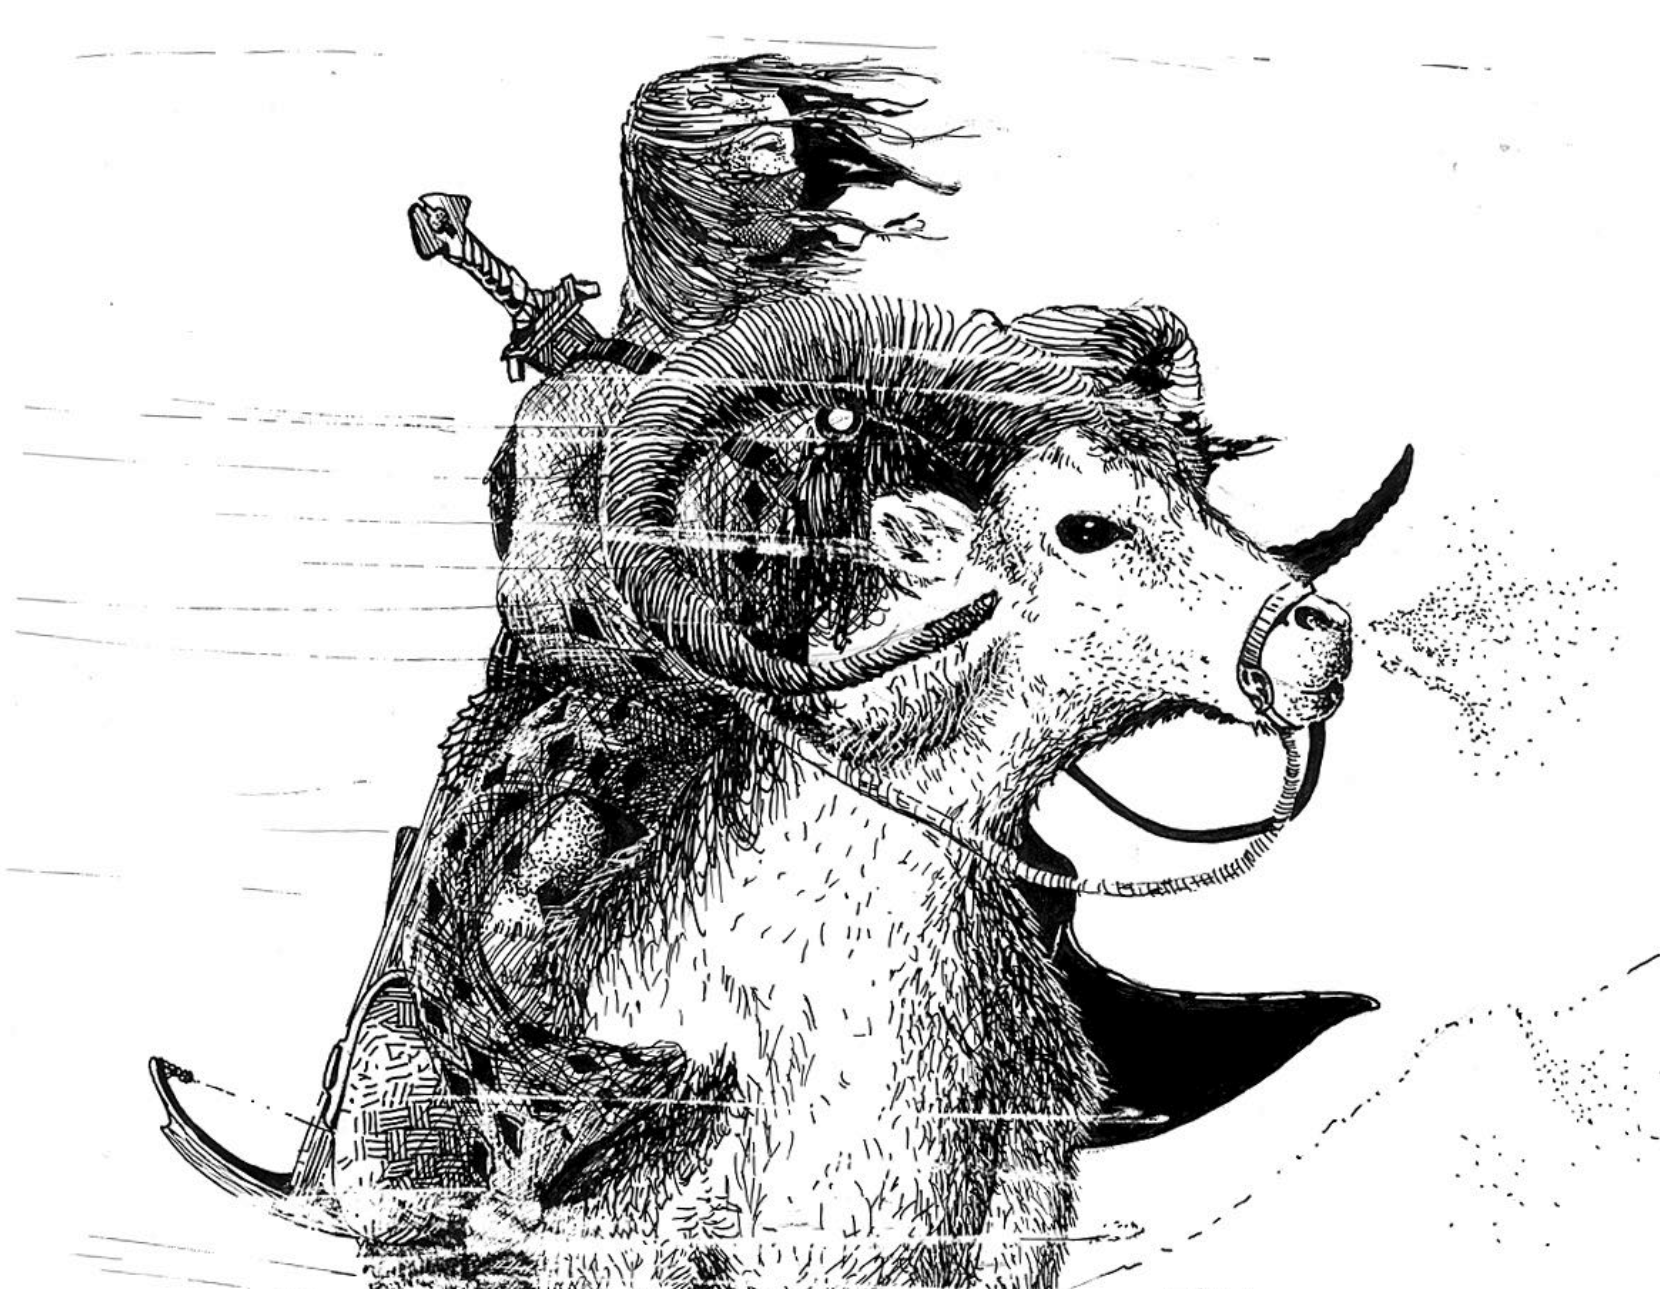
\includegraphics[width=1\linewidth,height=\textheight,keepaspectratio]{wanderer.png}
\caption{\emph{A ranger and their trusty steed}}
\end{figure}

\end{document}